\documentclass[11pt]{article}

\usepackage{threeparttable}
\usepackage{subfig}
\usepackage{pdfpages}
\usepackage{amsfonts,amsthm,amssymb,amsmath}
\usepackage{graphicx,mathrsfs}
\usepackage{multirow}
\usepackage{float}
%\usepackage{tikz}
%\usetikzlibrary{arrows}
\usepackage[hidelinks=true]{hyperref}
\usepackage{natbib}
\bibliographystyle{chicago}
%
% page format
\usepackage[top=0.81in,bottom=0.81in,left=0.81in,right=0.81in%,a4paper
]{geometry}
\linespread{1.3}
\setlength{\parskip}{3.6pt}

%% for cross reference in paper
%\usepackage{hyperref}
%\hypersetup{colorlinks,citecolor=black,filecolor=black,%
%  linkcolor=black,urlcolor=black}

\newtheorem{thm}{Theorem}
\newtheorem{prop}{Proposition}
\newtheorem{assu}{Assumption}
\newtheorem{definition}{Definition}%[section]
\newtheorem{lemma}{Lemma}
\newtheorem{coro}{Corollary}
\newtheorem{example}{Example}
\newtheorem{fact}{Fact}
\newtheorem{conjecture}{Conjecture}
\newtheorem{alg}{Algorithm}
\newtheorem{rem}{Remark}
\newtheorem{fig}{Figure}

\newcommand{\rv}{random variable}
\newcommand{\bE}{\bf E}
\renewcommand{\Box}{\bigboxvoid}
\newcommand{\qeds}{$\qedsymbol $}
\newcommand{\R}{\mathbb{R}}
\newcommand{\Z}{\mathbb{Z}}
\newcommand{\cc}{\mathbb{c}}

 %Natbib setup for author-year style

\title{\textbf{Authors' Reply\\Lagrangian Heuristic for Simultaneous Subsidization and Penalization:\\
Implementations on Rooted Travelling Salesman Games}}
\author{Lindong Liu, Yuqian Zhou, Zikang Li}
\date{}
\begin{document}
\maketitle

\noindent

We would like to thank the Associate Editor for processing our submission efficiently and providing guidance for the revision, and also thank the Referees for the encouraging and detailed comments on the paper.
We have carefully studied all the comments and addressed them in our manuscript.

% In this reply, we summarize several major changes we have made, and then give the specific details.
%
% First, regarding the equality in (4) is replaced to >= inequality in (6), we add a more detailed explanation. Meanwhile we explain that LP(4) is not a restriction of LP(2) in Reply 1 to Referee 1, maybe the term 'restricted LP' on page 7 caused the misunderstanding and we now use 'variant' to replace 'restricted'.
%
% Second, regarding the upper bound $c_u(V)$, we forgot to mention how to obtain the upper bound.
% In fact, all the upper and lower bounds of $c(S)$ are obtained by the Lagrangian relaxation method to keep the consistency and continuity.
%
% Third, regarding the proofs of Theorem 1 and Remark 1, we now add a clarification on the negative cost allocation in Reply 3 to Referee 1 and another clarification on the meaning of "the point-wise maximum of a finite set of straight lines".
%
%
% Fourth, regarding the sub-gradient method, we add a detailed clarification on page 9 including how the initial values of Lagrangian multipiers are given and how they change during the sub-gradient method.
%
%
% Fifth, regarding the symmetry of TSP game and why the TSP game is defined on the complete graph in our manuscript, we make the corresponding explanation in Reply 8 and Reply 6.
%
% Sixth, regarding the Figure 2, we add the definitions of squared points and round points to the legend of the figure and the meaning of curves (a) and (c) in Figure 2 is explained on page 17.
%

Please find below our point-by-point reply to each of the Referees. To facilitate reading, the original comments are in {\it italics}.

%\vspace{10mm}
\newpage

\noindent \textbf{\large Reply to Referee 1}
\\[3mm]
We appreciate your detailed comments.
We have carefully studied the technical concerns you raised, and revised our manuscript accordingly.
One thing we need to mention is that we have changed the notation of coalitions, $s$, to the standard form, $S$, according to the suggestion of  Referee 2.
The main issues raised in your report are addressed as follows:
\\[4mm]
%
%
\noindent \textit{\textbf{Question 1.}
Constraint \# 2 in problem (4). It appears from the next page that the equality can be replaced to $\geq$ inequality in this problem formulation. I would like the authors to expand the discussion of reasons for that being the case as the brief explanation on page 9 does not seem sufficient. Moreover, it looks like a good idea to do it right after introduction of problem (4), since in this case it becomes obvious that (4) is a restriction of (2) and therefore $z_r(w)$ is an upper bound on z(w):}
$$\beta(S) \leq c_l(S) + z \leq c(S) + z$$
$$\beta(V) \textcolor{red}{\geq c_u(V) + z \geq c(V) + z}$$
{\small Note: According to your context, there may be some typos in your comments, and they are now revised in red.}

\noindent \textbf{Reply 1.}
Thanks for your question. With regard to the conversion from the equality to the inequality, we have added more detailed explanations on page 9. For the second part of this question, we are sorry that the original term ``restricted LP" on page 7 is misunderstanding, and it is now replaced with term ``variant LP" to describe the relationships between LPs (2) and (4).

To be specific, when $c(S)$ and $c(V)$, in LP (2), are respectively replaced by $c_l(S)$ and $c_u(V)$ in LP (4).
Constraint $\beta(S) \leq c_l(S) + z \leq c(S) + z$ for any $S$ is a restriction of the original one, while $\beta(V) \geq c_u(V) + z \geq c(V) + z$ is not.
Therefore, LP(4) can be viewed as a variant, rather than a restriction, of LP(2).
Under the joint effects of the replacement of both constraints, we can find that LP(4) indeed can provide an upper bound for LP(2), as we have shown in Theorem 1.
\\[4mm]
%
%
%
\noindent \textit{\textbf{Question 2.}
When approximate problem (4) is introduced, it is not mentioned which upper bound $c_u(V)$ is used. Probably a discussion of upper bound possibilities will be good here.}
\\[2mm]
\noindent \textbf{Reply 2.}
Thanks a lot for your suggestion. 
In the first half of this manuscript, we are trying to introduce a general framework of computing feasible subsidy-penalty pairs under which the grand coalition is stabilized.
Therefore, the upper bound $c_u(V)$ in LP(4) could be any value larger than $c(V)$.
It could be either named by some authority, or computed by some well known heuristic algorithm (such as the linear relaxation based heuristics).
In the second half of this manuscript, when the Lagrangian relaxation technique is applied for approximation, $c_u(V)$ is obtained by a Lagrangian relaxation based heuristic for the sake of consistency and generality.
\textcolor{red}{We have added this clarification on page 7.}
% In fact, there are specific methods, such as LP-based methods, which can be used to obtain the upper bound $c_u(V)$.
% We have explicitly mentioned this in the paper.
% In order to be consistent with the general methods, we only mentioned a general method, i.e., Lagrangian heuristic to calculate the upper bound $c(V)$.
~\\[4mm]
%
%
%
\noindent \textit{\textbf{Question 3.}
Proof of Theorem 1. This is probably a general question but it also directly affects the proof of Theorem 1. The vector of cost allocation beta is defined to be in $R^v$.
I would like to see some discussion on why some individual cost allocation is allowed to be negative (implying a gain for a player, I guess) and how that is possible with existence of grand coalition. My concern is that beta components in the proof of Theorem 1 can become negative, but, again, I am not sure I understand the meaning of negative cost allocation.}
\\[2mm]
\noindent \textbf{Reply 3.}
%The main contributions are strengthened as explained in the first page of this reply.
Thanks for your question. 
Yes, as you have pointed out, when the cost assigned to some player is negative, it can be regarded as a gain for this player.

In fact, this phenomenon is not rare in the literature of ``Transferable Utilities (TU)" cooperative game theory (see, e.g., Caprara and Letchford 2010, Schulz and Uhan 2010).
And it can be physically done by transfer utilities among the players.
As long as each player is coalitionally beneficial, the cooperation is stable even though some player needn't to pay. 

We in addition need to point out that out main results still hold if $\beta$ is required to be positive.
Thanks a lot for raising this concern, which is helpful to improve the contents of this manuscript.
% The beta components in the proof indeed can be negative as you said, that is because the vector of cost allocation which is defined to be in $R^v$ in the proof is mathematically valid.
\\[4mm]
%\textcolor{blue}{
%The main contributions are strengthened as explained in the first page of this reply.
%We have tried our best to shorten the paper.
%There are 25 pages (excluding the reference) in the main part of the revision, while the results are more enriched and compact.
%We hope this is acceptable.}
%\\[4mm]
%
%
\noindent \textit{\textbf{Question 4.}
Proof of Remark 1. I am not able to see ``the point-wise maximum of a finite set of straight lines (hyperplanes, you mean?)" in defining the $z_r(w)$ (19). Please clarity.}
\\[2mm]
\noindent \textbf{Reply 4.}
Thanks a lot for your question. In the objective function of LP(19), each function 
$$\rho_v \big[ c_u(V)-\omega \big] - \sum_{S \in \mathbb{S} \setminus \{V\}} \rho_s c_l(S)$$
can be viewed as a straight line in $\omega$ whose slope is simply $-\rho_v$.
Hence, given some specific $\omega_0$, the value of $z_r(w_0)$ is the maximum of $\big\{\rho_v \big[ c_u(V)-\omega_0 \big] - \sum_{S \in \mathbb{S} \setminus \{V\}} \rho_s c_l(S):~\rho \in \text{feasible region of LP(19)} \big\}$.
This makes $z_r(w)$ be a point-wise maximum of straight lines $\rho_v \big[ c_u(V)-\omega \big] - \sum_{S \in \mathbb{S} \setminus \{V\}} \rho_s c_l(S)$.
\\[4mm]
%
%
%
\noindent \textit{\textbf{Question 5.}
In the description of the Algorithm 1, how is the initial restricted coalition set is constructed? For example, it is not clear what the first step means means if no initial set is defined. And also, I am not able to see how the initial values of Lagrangian coefficients lambda is constructed and how they change (if they do) during the algorithm. It would be great to add some clarifications.}
~\\[2mm]
\noindent \textbf{Reply 5.}
\textcolor{red}{I did not revise this paragraph}
Thanks for your question. Firstly, the initial restricted coalition set can be selected arbitrarily according to the column generation technique. Commonly we select the set which we think can help to accelerate computation speed. In this case, the restricted coalition set $S'$ is set to be $\{\{1\},\{2\},\ldots, \{v\}\}$, which can also be other forms.
Secondly, about the part of sub-gradient method, we have added the detailed clarification on page 9.
\\[4mm]
%
%
\noindent \textit{\textbf{Question 6.}
The description of the TSP game is somewhat different from one can find in the literature. For example in Tamir (1989) the game was defined on an uncomplete graph, while here the game is defined on the complete graph. This affects all the models presented on page 13 and further. Probably both versions of the game exist, but I would like to understand why the descriptions are different.}
~\\[2mm]
\noindent \textbf{Reply 6.}
Thanks a lot for your question. 
In fact we find that Tamir (1989) mentioned that the game was also equivalently defined on the complete graph in Potters et al. (1992).

We should admit that we chose complete graph for implementation since the resulting descriptions are consistent with our previous studies.
As far as we can see, by imposing large values of transportation cost, our complete-graph-model can also solve the problem when the graph is incomplete, while not vice versa.
% There is another change mainly for the convenience of presentation.
% For the **, we now define it as ** instead of **.
\\[4mm]
\noindent \textit{\textbf{Question 7.}
Constraint (15): I am not sure why would one keep (15) in such an aggregated format when it is possible to disaggregate it to $x_{ij} \leq \gamma_i$, $x_{ij} \leq \gamma_j$. In terms of LP relaxation disaggregation gives a tighter bound and probably will lead to the improvement to Lagrangian relaxation just as well.}
\\[2mm]
\noindent \textbf{Reply 7.}
Thanks a lot for your suggestion.
Yes, your are totally correct. The disaggregated format indeed gives a better bound when using LP relaxation.
However, in the context of Lagrangian relaxation, we thinks they are equivalent since we won't relax the integral constraint of $x_{ij}$.

For better understanding, we have changed the aggregated format to the disaggregated one you proposed, thanks again for your kind suggestion.
\\[4mm]
\noindent \textit{\textbf{Question 8.}
The symmetry of TSP game. I would like to attract the attention of the authors to the Dantzig Fulkerson Johnson (1954) paper, which originated the development of the TSP theory. Most importantly, the authors there also considered a symmetric TSP problem. If the problem is symmetric, one does not need as many binary variables as was introduced by authors. For example, on page 13 $x_{ij}$ exists together with $x_{ji}$ but direction of the travel is not important for symmetric problem therefore it is sufficient to introduce $x_e$ for e being an edge or $x_{ij}$ for $i < j$ only. This is how the TSP problem was introduced in DFJ and this is something that can simplify many notations in this paper. Also, it will be probably a good idea to get rid of $x_{ii}$ variables on page 13 and other optimization problems.}
~\\[2mm]
\noindent \textbf{Reply 8.}
Thanks a lot for your comment.
Yes, as you have pointed out, when it comes to a symmetric TSP problem, it is more convenient to introduce decision variables such as $``x_e"$ or $``x_{ij}, i<j"$.
However, in the context of cooperative game theory (e.g., TSP game), since we have to indicate the existence of some player in a coalition (e.g., $\gamma^{S}_j=1$ indicates that player $j$ is in coalition $S$), it would be useful and neat to introduce variable $x_{ij}$ for better descriptions.
\\[4mm]
\noindent \textit{\textbf{Question 9.}
I am a bit confused by Figure 2. Does it represent 4 different games? What exactly is on y axis and x axis, Penalty and Subsidy on y and x axis for all 4 figures? I suggest to add definitions of squared points and round points to the legend of the figure. Why is it that one figure gets two points and another gets 6 and they are evaluated at different levels of subsidy?}
~\\[2mm]
\noindent \textbf{Reply 9.}
Thanks for your suggestions. 
We are sorry for not making ourselves clear:
Figure 2 presents four representations of the curves of Lagrangian SPFs. The $x$ axis and the $y$ axis respectively represent the amount of subsidy and the amount of penalty in all 4 subfigures. We have added the definitions of squared points and round points into the legend of the figure.
\begin{figure}[H]
\centering
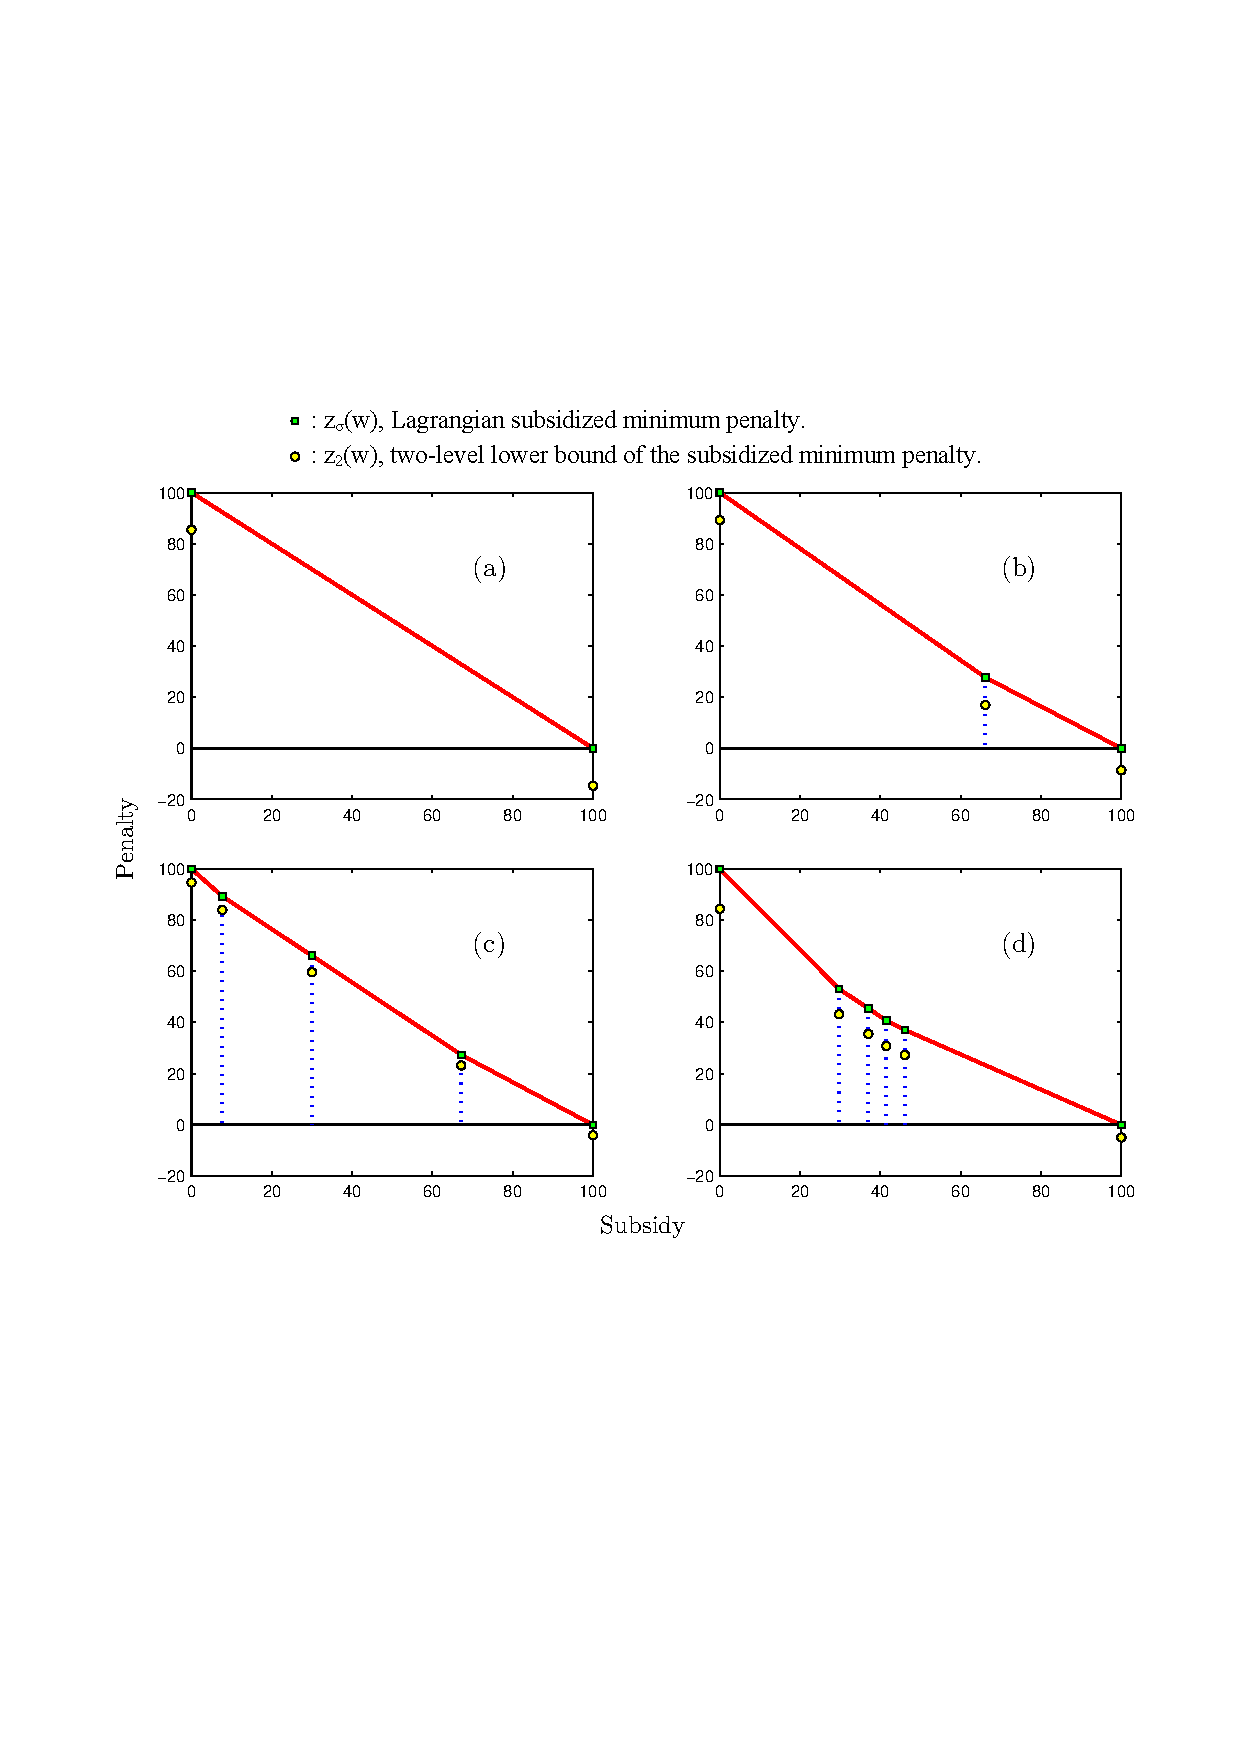
\includegraphics[width=1\textwidth]{1.pdf}
%\captionsetup{font={small}}
\centering
% \caption{\label{figure:20partitioned}Four representative Lagrangian SPFs for TSP games with 20 cities}
\end{figure}
\textcolor{red}{I did not revise this paragraph}
In addition, the meaning of curves (a) and (c) in Figure 2 is explained on page 17.
And the meaning of all curves in Figure 2 are shown below. (a) represents that the respective lines passing the two squared points have the same slope, thus there is no breakpoint between them.
% (a) represents that the slopes at the two points are equal, thus there is no breakpoint between them.
(b) represents that the two lines passing the two squared points at the beginning and the end meets a point, besides, the value of $z_\theta(\omega)$ at x-coordinate value of the point equals the value of y-coordinate of the point which indicates that this point is a breakpoint, which is the middle squared one. (c) represents that the two lines passing the two squared points at the beginning and the end intersects a point under the third squared point. Then with x-coordinate value of this intersection point, the third squared point can be obtained by Algorithm 1 in our manuscript. With the IPC algorithm proposed by Liu et al. (2018), we can generate the line passing the third squared point. Finally, this line intersects the two lines passing the two points at the beginning and the end at the second and fourth squared points, respectively.
% (c) represents that the two lines passing the two points at the beginning and the end meets a point whose y-coordinate value is not equal to the third squared point's y-coordinate value, $z_\theta(\omega)$ at x-coordinate value of the point. The line passing the third squared point intersects the two lines passing the two points at the beginning and the end at the second and fourth squared points, respectively.
The difference of (c) and (d) is that (d) has one more line intersection process than (c) at the right half part of the subfigure.
~\\[4mm]
\noindent \textit{\textbf{Question 10.}
In regards to results of experiments in Table 3, what exactly was used and the upper bound $\phi(N)$? and finally a general remark on the lower bound construction z(w):
-- if we consider problem (4) as a restriction of (2), then it is also possible to create a relaxation of the problem in the similar was as problem (4) was constructed.}
\\[2mm]
\noindent \textbf{Reply 10.}
Thanks for your question. Firstly, the $\phi(N)$ is an upper bound of $c_t(N)$ obtained by the Lagrangian relaxation method as we have clarified in Reply 2.
% The upper bound $\phi(N)$ is what we use Lagrangian heuristic method to obtain.
Secondly, we are sorry for the misunderstanding term ``restricted LP" in the original manuscript.
As we have clarified in Reply 1, LP(4) is a variant, rather than a restriction, of LP(2).
% Based on the above analysis, LP(4) is not a restriction of LP(2), which can also explain why we cannot get a relaxation of LP(2) if we switch the places of $c_l(S)$ and $c_u(S)$ you mentioned in Question 10.
~\\[4mm]

% \noindent \textit{\textbf{Minor comments.}}

% 1. Problem (2) in the paper is frequently called an LP problem or a combinatorial optimization problem (page 4, for example). I suggest to use one terminology approach for consistency. For example, page 8 "solve LP (4) with some conventional combinatorial optimization techniques" sounds confusing.
%
% 2. Remark 1: probably, for any s in S \ V in the first line of the Remark?
%
% 3. Page 8, line 58. Perhaps it is worth mentioning that this is due to Lagrangian being concave function.
%
% 4. Page 10, line 60. Perhaps LP (4) instead of (2)?
%
% 5. Page 10, line 26. Perhaps, it is better to replace forward reference (9) by "reduced cost".
%
% 6. Page 13, I would suggest to make a reference to the Dantzig Fulkerson Johnson (1954) paper with respect to constraints (13), as these constraints are not given in TSP
% literature but are in fact result of development by those authors.
%
% 7. I would suggest merging first two constraints in (11) as it is a bit confusing in its present form.
%
% 8. Page 15, line 45. don't you need to remove the word 'minimum' here?}
%
% \\[2mm]

\noindent \textbf{Reply to Minor Comments.}
Thank you very much for pointing out the typos of our manuscript in Minor Comments. We have made corresponding revisions.


% 1. We have changed our expression use LP problem to avoid the confusion. according to the Minor comments
%
% 2. We've revised.
%
% 3. We have added the concave property before mentioning the sub-gradient method.

% 5. We've replaced (9) by 'reduced cost' to avoid the forward reference.
%
% 6. We've added a reference to the Dantzig Fulkerson Johnson (1954) paper when introducing constraints (13).
%
% 7. We've merged the first two constraints for the ease of understanding.
%
% 8. We've removed the word 'minimum'.
~\\[4mm]

%\vspace{10mm}
\newpage

\noindent \textbf{\large Reply to Referee 2}
\\[3mm]
Thank you very much for your appreciation of our work.
We have corrected all the typos and grammatical errors that you pointed out.
%As stated in the first two pages, we have made some major changes to the paper structure to strengthen the main contributions of our work.
%Sections 4 and 5 in the original paper are replaced.
%In this report, we will focus on responding to the comments which still mater in the current paper.
%Your other comments will be great helpful in our further study. Thanks a lot for your work.
~\\[4mm]
%
%
%
\noindent \textit{\textbf{Question 1.}
Notation. The paper does not conform with the standard notation in TU-games. Usually, coalitions are referred with capital letters and its cardinal in lower case letters, i.e. $S \subset N$ and $|S| = s$. This paper uses a different notation with $s$ for coalitions and then some inconsistencies appears when referring to $v$ in some places. I would suggest to adapt the notation to the standard to ease the readability of potential readers.}
~\\[2mm]
\noindent \textbf{Reply 1.}
Thanks a lot for your suggestion.
We have changed the notation to the standard form all over the revised manuscript.
\\[4mm]
%
%
%
\noindent \textit{\textbf{Question 2.}
Some confusion appears, here and there, when referring to LP or MIP.
For instance, on page 4 line 3, it is mentioned that (2) is a combinatorial optimization problem. However, (2) is a LP since in its description c is
given and thus all constraints and variables are linear and continuous.
The same confusion can be found at other places of the paper. Please clarify!}
\\[2mm]
\noindent \textbf{Reply 2.}
We have changed our expression by using only term ``LP"  to avoid the confusions.
\\[4mm]
%
%
%
\noindent \textit{\textbf{Question 3.}
Page 4 line -13: The authors must be more precise. The Lagrangean
bound is more accurate than the linear relaxation whenever the problem does not fulfill the integrality property.
}
\\[2mm]
\noindent \textbf{Reply 3.}
We are sorry for our aggressive statement, and thank you a lot for pointing this out.
We have added the pre-condition, ``for those integer linear programmings which do not fulfill the integrality property", to the manuscript on page 4.
%We have revised our wordings in line X of page X in the revised manuscript.
\\[4mm]
%
%
%
\noindent \textit{\textbf{Question 4.}
The statement of Theorem 1 should be modified since the value of the
LP is one of the many possible upper bounds not the only one as stated
there.
}
~\\[2mm]
\noindent \textbf{Reply 4.}
Yes, you are correct. It should be ``... value of LP(4) is \textcolor{red}{\bf an} upper bound of ...". Thanks for pointing this out.
~\\[4mm]
%
%
%
\noindent \textit{\textbf{Question 5.}
Remark 1. The meaning of $v$ is unclear. One should guess that it refers
to $|V|$ but this has to be made explicit.
}
\\[2mm]
\noindent \textbf{Reply 5.}
We have pointed this out in the revised manuscript on page 8.
\\[4mm]
%
%
%
\noindent \textit{\textbf{Question 6.}
Page 8, line -12. Note that (5) is not an LP but an ILP.
}
\\[2mm]
\noindent \textbf{Reply 6.}
Thank you for pointing this out.
This should be ILP.
\\[4mm]
%
%
%
\noindent \textit{\textbf{Question 7.}
To better illustrate the proposed methodology, it would be advisable
to apply it not only to the rooted traveling salesman problem. I would
suggest to add another class of combinatorial games, for instance location games, to the computational study.}
\\[2mm]
\noindent \textbf{Reply 7.}
Thanks again for your appreciation of our methodology.

Although our framework is sort of general, as you may have noticed, for different types of games, the resulting pricing problem (e.g., LP(18) for TSP game) varies a lot and often desires problem-specific solution approach.
To strengthen the focus of this manuscript, i.e., proposing general framework to solve subsidy-penalty pairs in stabilizing grand coalitions, it might be helpful to include only TSP game here for implementation.
In fact we have considered some other games for implementations before the first round of submission.
We believe that some implementations can lead to interesting results while beyond the scope of this manuscript.

Again, we are grateful for your constructive suggestion, and will try more implementations, including some new theoretical results, in the future research.
Hope this is acceptful for this round of revision.
% Maybe this method applied on another class of combinatorial game is time-consuming and beyond the scope of this manuscript.
\\[4mm]
%
%
%%%%%%%%%%%%%%%%%
\end{document}
%%%%%%%%%%%%%%%%%
